\subsection{Osservazioni}
Osserviamo il risultato su un'immagine scelta casualmente del set creato e sulle due immagini aggiuntive.
%! l'elemento principale e' il rumore + mettere confronti
\subsubsection{Analisi immagine geometrica}
Analizziamo l'immagine img8.png al variare del valore $\sigma$:

Ricordiamo che più è alto il valore del PSNR maggiore sarà la vicinanza dell'immagine corrotta rispetto alla versione originale. 

Le figure di sinistra rappresentano l'immagine originale, invece a destra sono riportate le immagini corrotte con i rispettivi valori di PSNR. 
Notiamo che all'aumentare delle dimensioni di sigma il valore di PSNR diminuisce che denota un peggioramento della qualità dell'immagine, 
infatti le immagini subiscono un'appiattimento dell'intensità della scala dei colori e i contorni delle varie figure geometriche perdono di fermezza. 
Inoltre è curioso notare.. %! da finire

\begin{figure}[H]
    \centering
    \begin{subfigure}{0.6\textwidth}
        \centering
        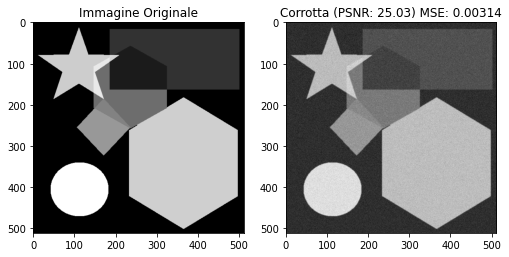
\includegraphics[width=\textwidth]{imgRel/img8corrotto/img8corrotta5x5.png}
        \caption{Img8 corrotta con $\sigma = 0.5$ dimensione $5 \times 5$}
        \label{fig: 8corrotto5}
    \end{subfigure}
    \begin{subfigure}{0.6\textwidth}
        \centering
        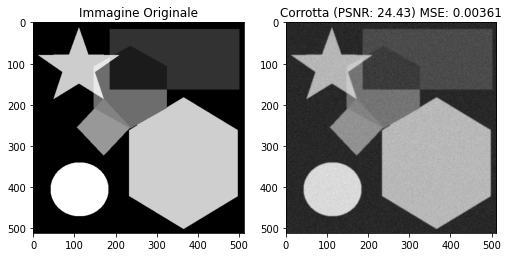
\includegraphics[width=\textwidth]{imgRel/img8corrotto/img8corrotta7x7.png}
        \caption{Img8 corrotta con $\sigma = 1$ dimensione $7\times 7$}
        \label{fig: 8corrotto7}
    \end{subfigure}
    \begin{subfigure}{0.6\textwidth}
        \centering
        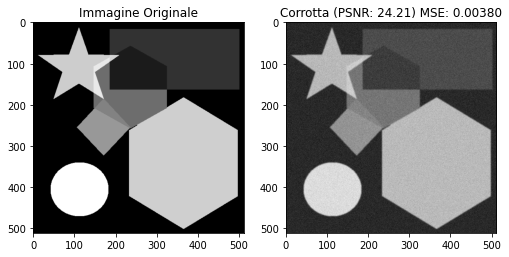
\includegraphics[width=\textwidth]{imgRel/img8corrotto/img8corrotta9x9.png}
        \caption{Img8 corrotta con $\sigma = 1.3$ dimensione $9 \times 9$}
        \label{fig: 8corrotto9}
    \end{subfigure}
    \caption{Immagine geometrica corrotta al variare di }
    \label{fig: 8corrotto}
\end{figure}

\subsubsection{Analisi immagine fotografica}
Si nota un'altra volta che all'aumentare delle dimensioni di $\sigma$ diminuisce il PSNR e l'immagine perde di 
incisività, le versioni corrotte benché risultino visivamente peggiori, si riesce ancora a ben distinguere il 
soggetto in primo piano, anche se sfocato, in tutte le immagini. 

\begin{figure}[H]
    \centering
    \begin{subfigure}{0.6\textwidth}
        \centering
        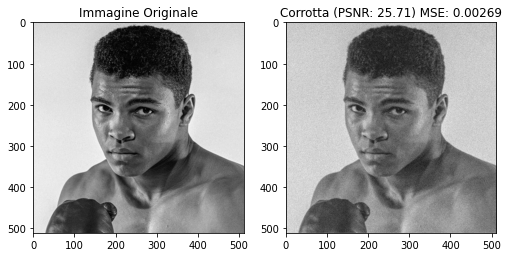
\includegraphics[width=\textwidth]{imgRel/muhammedcorrotto/muhammedcorrotto5x5.png}
        \caption{Pugile.png corrotta con $\sigma = 0.5$ dimensione $5 \times 5$}
        \label{fig: pugilecorrotto5}
    \end{subfigure}
    \begin{subfigure}{0.6\textwidth}
        \centering
        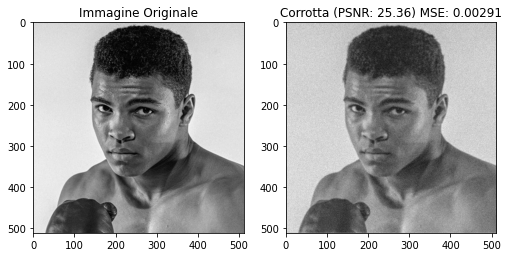
\includegraphics[width=\textwidth]{imgRel/muhammedcorrotto/muhammedcorrotto7x7.png}
        \caption{Pugile.png corrotta con $\sigma = 1$ dimensione $7 \times 7$}
        \label{fig: pugilecorrotto7}
    \end{subfigure}
    \begin{subfigure}{0.6\textwidth}
        \centering
        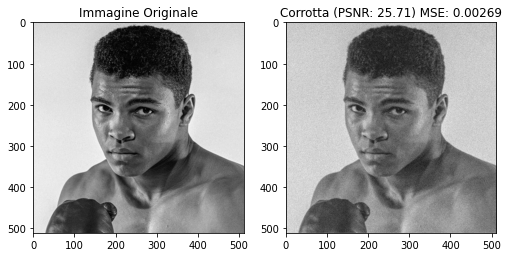
\includegraphics[width=\textwidth]{imgRel/muhammedcorrotto/muhammedcorrotto5x5.png}
        \caption{Pugile.png corrotta con $\sigma = 1.3$ dimensione $9 \times 9$}
        \label{fig: pugilecorrotto9}
    \end{subfigure}
    \caption{Immagine fotografica corrotta al variare di $\sigma$}
    \label{fig: PugileCorrotto}
\end{figure}

\subsubsection{Analisi immagine con testo}
In questa immagine abbiamo una raccolta di prime pagine di giornale che ci permettono di osservare e valutare 
meglio la differenza tra l'immagine originale e la versione corrotta, per esempio con $\sigma = 0,5$ (vedi immagine \ref{fig: giornalecorrotto5}) 
otteniamo un'immagine con del testo ancora leggibile sebbene meno nitida, la difficoltà inizia ad essere maggiore invece con 
$\sigma = 1$ (vedi immagine \ref{fig: giornalecorrotto7}) dove le scritte più piccole diventano quasi illeggibili, con $\sigma = 1.3$ 
(vedi immagine \ref{fig: giornalecorrotto9}) il PSNR diminuisce ancora sebbene non molto rispetto rispetto a sigma uguale a 1, ma in questo caso anche le scritte più grandi, fatta 
eccezione per i titoli, perdono di chiarezza. 
\begin{figure}[H]
    \centering
    \begin{subfigure}{0.6\textwidth}
        \centering
        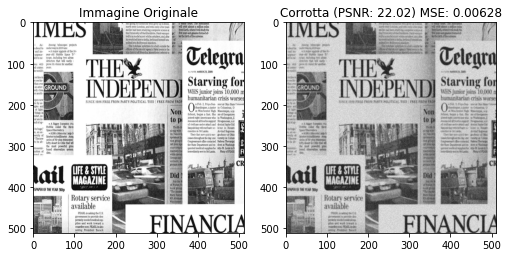
\includegraphics[width=\textwidth]{imgRel/testocorrotto/testocorrotto5x5.png}
        \caption{giornale.png corrotta con $\sigma = 0.5$ dimensione $5 \times 5$}
        \label{fig: giornalecorrotto5}
    \end{subfigure}
    \begin{subfigure}{0.6\textwidth}
        \centering
        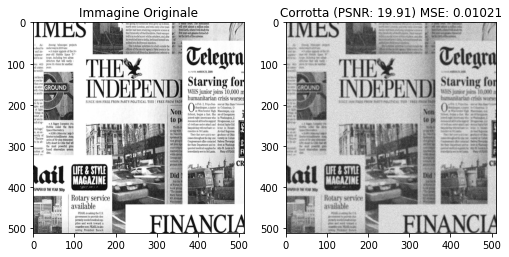
\includegraphics[width=\textwidth]{imgRel/testocorrotto/testocorrotto7x7.png}
        \caption{giornale.png corrotta con $\sigma = 1$ dimensione $7 \times 7$}
        \label{fig: giornalecorrotto7}
    \end{subfigure}
    \begin{subfigure}{0.6\textwidth}
        \centering
        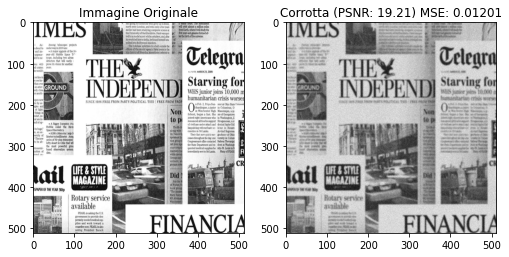
\includegraphics[width=\textwidth]{imgRel/testocorrotto/testocorrotto9x9.png}
        \caption{giornale.png corrotta con $\sigma = 1.3$ dimensione $9 \times 9$}
        \label{fig: giornalecorrotto9}
    \end{subfigure}
    \caption{Immagine con testo corrotta al variare di $\sigma$}
    \label{fig: GiornaleCorrotto}
\end{figure}